\begin{figure}[ht]
\centering
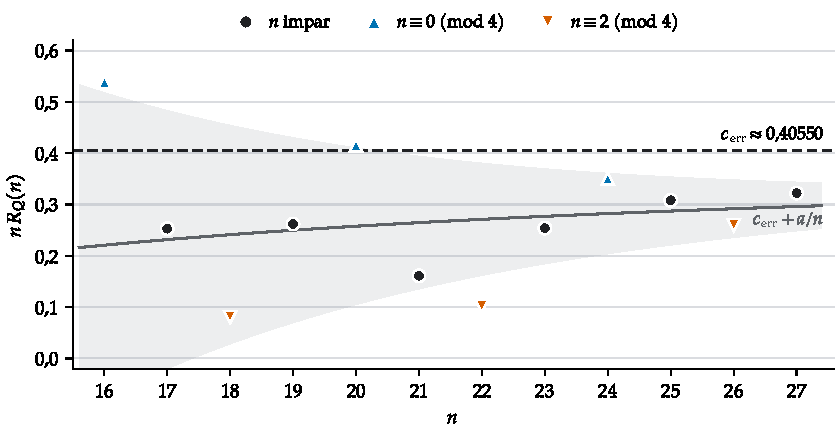
\includegraphics[width=.9\linewidth]{figuras/conteos.pdf}
\caption{Valores de $nR_Q(n)$ para $16\le n\le27$, obtenidos de los conteos exactos y del predictor
canónico (evidencia numérica). La línea discontinua marca el valor de $\cerr$ obtenido del continuo
y fijado antes del ajuste a estos doce tamaños. La curva gris
muestra la deriva ajustada $\cerr+a/n$, con $a\simeq-2{,}956$, y la banda sombreada tiene la amplitud
$Ae^{-\kappa(n-16)}$ de la oscilación de periodo cuatro (Apéndice~\ref{app:numquad}). Los tamaños
impares tienen oscilación ajustada cero. En los tamaños pares el modelo suma esa amplitud
si $n\equiv0\;(\mathrm{mod}\,4)$ y la resta si $n\equiv2\;(\mathrm{mod}\,4)$.}\label{fig:counts}
\end{figure}
